\chapter{Tests}
\section{Android JUnit Test}
Android propose un framework permettant d'effectuer nos propre tests unitaire.
Pour ce faire nous avons créé un nouveau projet de type \textit{Android Test Project}. Toute classe de test de ce projet devra heriter de la classe \textit{TestCase} (ou d'une des ses sous-classes) pour permettre l'initialisation du téléphone. Puis nous avons surchargé la methode \textit{setUp} afin de definir l'etat du téléphone à l'instant où le test est lancé.
\begin{lstlisting}[format=JAVA]
    @Override
    protected void setUp() throws Exception {
	super.setUp();
	mActivity = this.getActivity();
	src = new Camera("test", "root", "root", "192.168.1.20", 80, "http", 1);
    }
\end{lstlisting}

Une fois ces étapes réalisées, nous pouvons implémenter l'ensemble de nos tests unitaire dans des fonctions distinctes. Nous avons choisis de tester septs fonction de notre projet :
\begin{enumerate}
\item Le premier test a pour but de tester l'ajout de plusieurs caméras, puis dans le cas où cette étape reussie, d'exporter les caméras, de vider la liste et de les réimporter afin d'observer d'éventuel dysfonctionnements.
\begin{lstlisting}[format=JAVA,caption={Test 1 : Import/Export}]
  public void testimport() {
	/* Ajout 3 cameras */
	camList = new ArrayList<Camera>();
	int position = camList.size();
	src.setUniqueID(position);
	camList.add(position, src);
	assertEquals(camList.size(), 1);

	position = camList.size();
	src.setUniqueID(position);
	camList.add(position, src);
	assertEquals(camList.size(), 2);

	position = camList.size();
	src.setUniqueID(position);
	camList.add(position, src);
	assertEquals(camList.size(), 3);

	/* Export */
	boolean res = xmlIO.xmlWrite(camList, exportPath, exportName);
	assertEquals(res, true);

	/* Purge la liste */
	camList.clear();
	assertEquals(camList.size(), 0);

	/* Import */
	camList = xmlIO.xmlRead(exportPath + exportName);
	assertEquals(camList.size(), 3);
    }
\end{lstlisting}
\item Le second test porte sur l'ajout d'une notification dans la barre de notification, puis de sa suppression. Ce test require la presence de l'utilisateur pour observer les resultats, en effet, durant le test precedent la presence d'\textit{assert} nous garanti le resultat. Ici c'est l'observation de l'apparition d'une notification qui nous permet de constater la reussite du test.
\begin{lstlisting}[format=JAVA,caption={Test 2 : Notification}]
    public void testNotification() {
	/* ajout notif */
	int index = 5;
	Resources res = mActivity.getResources();
	Drawable drawable = res
		.getDrawable(com.myapps.R.drawable.hello_android);
	Bitmap bmp = ((BitmapDrawable) drawable).getBitmap();
	notificationLauncher.statusBarNotificationImage(mActivity, bmp, "test",
		"blabla", index, "tag");
	NotificationManager notificationManager;
	notificationManager = (NotificationManager) mActivity
		.getSystemService(Context.NOTIFICATION_SERVICE);
    }
\end{lstlisting}
\item Le troisieme test ressemble au second à l'exception que celui-ci test les notification dite \textit{En Cours}.
\begin{lstlisting}[format=JAVA,caption={Test 3 : Notification En-Cours}]
  public void testRunningNotification() {
	int index = 10;
	Intent notificationIntent = new Intent(
		mActivity.getApplicationContext(), Video.class);

	Bundle objetbunble = new Bundle();
	objetbunble.putSerializable(
		mActivity.getString(com.myapps.R.string.camTag), src);
	notificationIntent.putExtras(objetbunble);
	notificationIntent.setAction(Intent.ACTION_MAIN);
	/* Ajout de data inutile pour l'application mais necessaire pour que la fonction filterEquals() retourne faut pour deux intents avec des extras differents */
	notificationIntent.setDataAndType(Uri.parse("value"), "Camera");
	PendingIntent contentIntent = PendingIntent.getActivity(
		mActivity.getApplicationContext(), 0, notificationIntent, 0);
	notificationLauncher
		.statusBarNotificationRunning(mActivity.getApplication(),
			contentIntent, index, "ca tourne !");

	notificationLauncher.removeStatusBarNotificationRunning(
		mActivity.getApplication(), index);
    }
\end{lstlisting}

\end{enumerate}
Nous allons maintenant passer aux fonctions de contrôle ainsi qu'aux services fourni par la caméra :
\begin{enumerate}
  \setcounter{enumi}{4}
  \item Nous allons commencer par un simple test nous permettant de verifier l'etablissement d'une connection lors de l'appel à la fonction \textit{sendCommand}. L'assert nous permet de garantir l'etablissement de la connection quelque soit le resultat de la requette.
\begin{lstlisting}[format=JAVA,caption={Test 4 : Connection HTTP}]
   public void testSendCommand() {
	CameraControl c = new CameraControl(src, mActivity);
	HttpURLConnection res = null;
	try {
	    res = c.sendCommand("axis-cgi/com/ptz.cgi?info=1&camera=1");

	} catch (IOException e) {
	    e.printStackTrace();
	}
	assertNotNull(res);
    }
\end{lstlisting}

\item La garantie du test précédent nous permet d'effectuer des tests de plus en plus precis. Ce 5eme test a pour but de tester la prise de photo instantannée ainsi que la sauvegarde de celle-ci sur la carte mémoire. Afin de constater que la caméra nous a bien envoyer la bonne photo, l'utilisateur peut la visionner dans le dossier \textit{"/sdcard/com.myapps.camera/"}.
\begin{lstlisting}[format=JAVA,caption={Test 5 : SnapShot et sauvegarde}]
 public void testSnap() {
	CameraControl camC = new CameraControl(src, mActivity);
	String[] resolutions = camC.getResolutions();
	String fileNameURL = "/sdcard/com.myapps.camera/";
	String fileName = "Snap-" + System.currentTimeMillis() + ".jpeg";
	Bitmap bmp;
	try {
	    bmp = camC.takeSnapshot(resolutions[0]);
	    assertNotNull(bmp);
	    snapShotManager.saveSnap(bmp, fileNameURL, fileName);
	} catch (IOException e) {
	    e.printStackTrace();
	}
    }
\end{lstlisting}

\item La détection de mouvement fait necessite l'interaction entre une activité et un service lors de son lancement, c'est pourquoi nous avons testé séparement l'ajout et la suppression d'une fenetre de la detection en elle meme comme le montre les deux tests suivant. Le premier de ces deux test verifie que la caméra retourne bien le numéro de groupe attribué à la fenetre. Si celui-ci est correct, l'assert ne se declanche pas, on peut alors liberer la fenetre de la caméra.
\begin{lstlisting}[format=JAVA,caption={Test 6 : Ajout et suppression d'une fenetre}]
 public void testAddRemoveMotionDetection() {
	CameraControl c = new CameraControl(src, mActivity);
	assertNotNull(c);
	int groupe = -1;
	try {
	    groupe = c.addMotionD();
	    assertNotSame(groupe, -1);

	    groupe = c.removeMotionD();
	    assertEquals(groupe, -1);
	} catch (IOException e) {
	    e.printStackTrace();
	} catch (CouldNotCreateGroupException e) {
	    e.printStackTrace();
	}
    }
\end{lstlisting}
\item Ce dernier test est probablement le plus important de cette partie. Si il termine, il permet de constater le déclanchement de la notification lors de la capture d'un mouvement (snapshot plus vibration du téléphone). L'idée est de mettre en route la detection de mouvement sur la caméra \textit{src} (fenetre par defaut). Une fois celle-ci lancée, nous faisons boucler le programme tant que la caméra ne detecte pas de mouvements. Si un mouvement est détecté, le processus sort de la boucle, puis stoppe la détection nous garantissant la présence d'un mouvement.

\begin{lstlisting}[format=JAVA,caption={Test 7 :Détection des mouvements}]
    public void testMD() {
	try {
	    CameraControl c = new CameraControl(src, mActivity);
	    int group = c.addMotionD();
	    c.cam.setGroup(group);
	    
	    Intent intent = new Intent(mActivity, MotionDetectionService.class);
	    Bundle objetbunble = new Bundle();
	    objetbunble.putSerializable(mActivity.getString(R.string.camTag),
		    c.cam);
	    intent.putExtras(objetbunble);
	    int lim = 20;
	    long delay = 1000;
	    intent.putExtra("limit", lim);
	    intent.putExtra("delay", delay);
	    mActivity.startService(intent);
	    while(MotionDetectionService.detected == false){
		Thread.sleep(1000);
		/* passer devant la cam pour continuer */
	    }
	    
	    int indice;
	    if ((indice = MotionDetectionService.isAlreadyRunning(c.cam)) != -1) {
		MotionDetectionService.stopRunningDetection(c.cam,
			mActivity.getApplication(), indice);

		c.removeMotionD();
	    }

	} catch (IOException e) {
	    e.printStackTrace();
	} catch (CouldNotCreateGroupException e) {
	    e.printStackTrace();
	} catch (InterruptedException e) {
	    e.printStackTrace();
	}

    }

\end{lstlisting}
\end{enumerate}


\section{Analyse des connections via WireShark}
Grace au périphérique virtuel fournit dans le sdk d'Android, nous sommes en
mesure d'analyser le trafic entre la caméra et le périphérique (téléphone ou
tablette). Pour ce faire nous avons utilisé le logiciel
\textit{Wireshark}\footnote{\label{Wireshark}http://www.wireshark.org/}.\newline
Grace au trafic enregistré par Wireshark nous avons pu constater que :
\begin{itemize}
  \item L'ensemble des connections ouverte sont correctement fermées grace
  l'utilisation de la fonction \textit{disconnect()} definie par la classe \textit{HttpURLConnection}.
  L'exemple ci-dessus represente le demarrage d'une simple vue pour la caméra d'adresse
  \textit{192.168.1.20}. Pour effectuer ce test nous avons ralenti l'execution
  de l'application afin d'éviter l'entrelassement des paquets. On retrouve les
  deux connections permettant la récupération des informations relative à la
  caméra (connections 51576 et 51577), ainsi que la demande du flux vidéo
  (connection 51578). La présence du second paquet 
  fin ainsi que son acquitement n'apparaissent pas sur la capture dut à la
  latence engendré par la fermeture et la liberation des sockets/ressources.
\begin{center}
 \begin{figure}[H] 
  \label{finConnection}
  \centering
  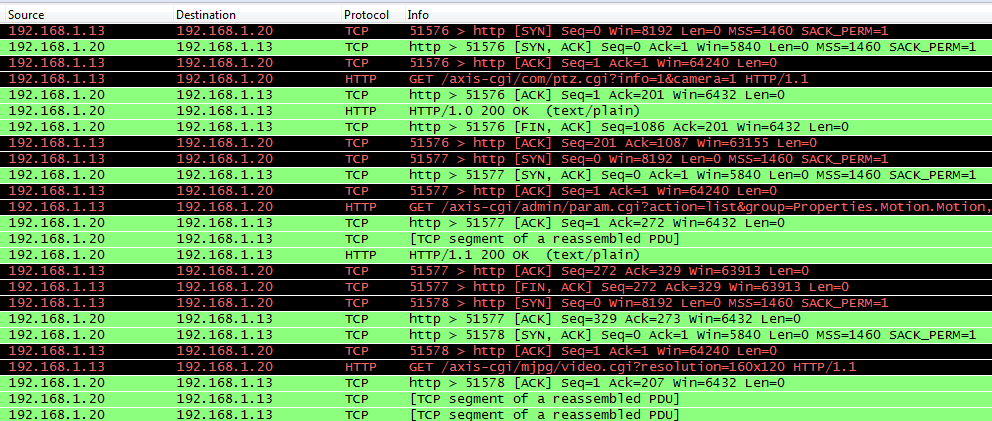
\includegraphics[scale=0.6]{Images/finConnection.png}
  \caption{Wireshark capture}
\end{figure}  
\end{center}

  \item Notre PlayerThread reduit considerablement la consomation de la bande
  passante au detriment des fps. Exemple : la comparaison de deux capture sur un
  même interval de temps nous a permi d'effectuer une comparaison du nombre de
  paquet echangé ainsi que leurs taille.
  \item En supplément du test numéro 7,  nous observons que le service mi en
  place pour la détéction de mouvement continue à echanger des informations avec
  la caméra malgres la fermeture de l'application. 
\end{itemize}
\section{Manipulation avec la caméra}
La derniere phase de test consiste à verifier la totalité des services fourni
par l'application en observant les effets sur la caméra.\newline
Nous avons grace à cela verifier que :
\begin{itemize}
  \item La totalité des controles (PTZ) implémentés correspondent aux mouvements
  de la caméra.
  \item Les fonctions de controle avancé sur la vidéo s'activent correctement.
  \item La détéction de mouvements se declanche correctement (en adéquation
  avec les test precedents)
  \item La vidéo observée sur le téléphone correspond à la zone pointée par la
  caméra (en fonction de la vue et des parametres
  utilisées ainsi que de la couverture réseaux).
\end{itemize}

